\section{\textit{Unified Modelling Language}}
Unified Modeling Language atau UML adalah bahasa pemodelan standar yang digunakan dalam rekayasa perangkat lunak untuk menspesifikasi, memvisualisasikan, mengembangkan, dan mendokumentasikan artefak sistem perangkat lunak. UML menyediakan serangkaian teknik notasi grafis untuk membuat model visual dari sistem perangkat lunak berorientasi objek. UML mencakup berbagai jenis diagram, termasuk diagram struktural (seperti diagram kelas dan diagram komponen) dan diagram perilaku (seperti diagram ``use case'' dan ``sequence diagram''), yang membantu dalam memahami arsitektur dan perilaku sistem \citep{huzar2005uml}.
\singlespacing{}
UML banyak diadopsi dalam industri karena kemampuannya memfasilitasi komunikasi antar pemangku kepentingan, termasuk pengembang, desainer, dan analis bisnis, dengan menyediakan bahasa umum untuk memodelkan sistem yang kompleks \citep{huzar2005uml}.
\singlespacing{}
UML terdiri dari sejumlah diagram yang telah distandardisasi untuk pengembangan perangkat lunak berbasis objek, menjadikannya alat berharga untuk pemodelan dan desain sistem \citep{weriza2022development}. Dalam penulisan ini penulis menggunakan 2 macam jenis di antaranya:

\subsection{Use Case Diagram}
Diagram ``use case'' adalah jenis diagram perilaku dalam Unified Modeling Language (UML) yang merepresentasikan kebutuhan fungsional dari suatu sistem. Diagram ini menggambarkan interaksi antara pengguna (aktor) dan sistem itu sendiri, menangkap berbagai cara di mana sistem dapat digunakan. Diagram ``use case'' membantu mengidentifikasi fungsionalitas sistem dan hubungan antara berbagai ``use case'', memberikan gambaran umum tentang perilaku sistem.
\singlespacing{}
Dalam diagram ``use case'', aktor digambarkan sebagai figur tongkat, sementara ``use case'' diwakili sebagai oval. Garis menghubungkan aktor dengan ``use case'' yang mereka interaksikan, menunjukkan hubungan dan interaksi. Representasi visual ini membantu dalam memahami kebutuhan sistem dan berfungsi sebagai alat komunikasi di antara para pemangku kepentingan \citep{huzar2005uml}.
\singlespacing{}
Untuk memahami diagram kasus pengguna, penting untuk mengenali simbol-simbol yang digunakan. Simbol-simbol dalam diagram kasus pengguna termasuk:
\begin{itemize}
  \item Aktor, yang digambarkan dengan ikon manusia kecil, yang mewakili pengguna atau sistem lain yang berinteraksi dengan sistem yang dimodelkan.
  \item Kasus penggunaan, yang merepresentasikan fungsi atau layanan yang disediakan oleh sistem, digambarkan dengan elips.
  \item Hubungan antara aktor dan kasus penggunaan digambarkan dengan garis-garis yang menunjukkan interaksi.
  \item Hubungan ``extend'' dan ``include'' yang menunjukkan variasi atau ketergantungan dalam fungsionalitas.
\end{itemize}
Dengan memahami simbol-simbol ini, pengembang dapat lebih efektif dalam mendokumentasikan dan menganalisis kebutuhan sistem \citep{huzar2005uml}.

\begin{figure}[htbp]
  \centering
  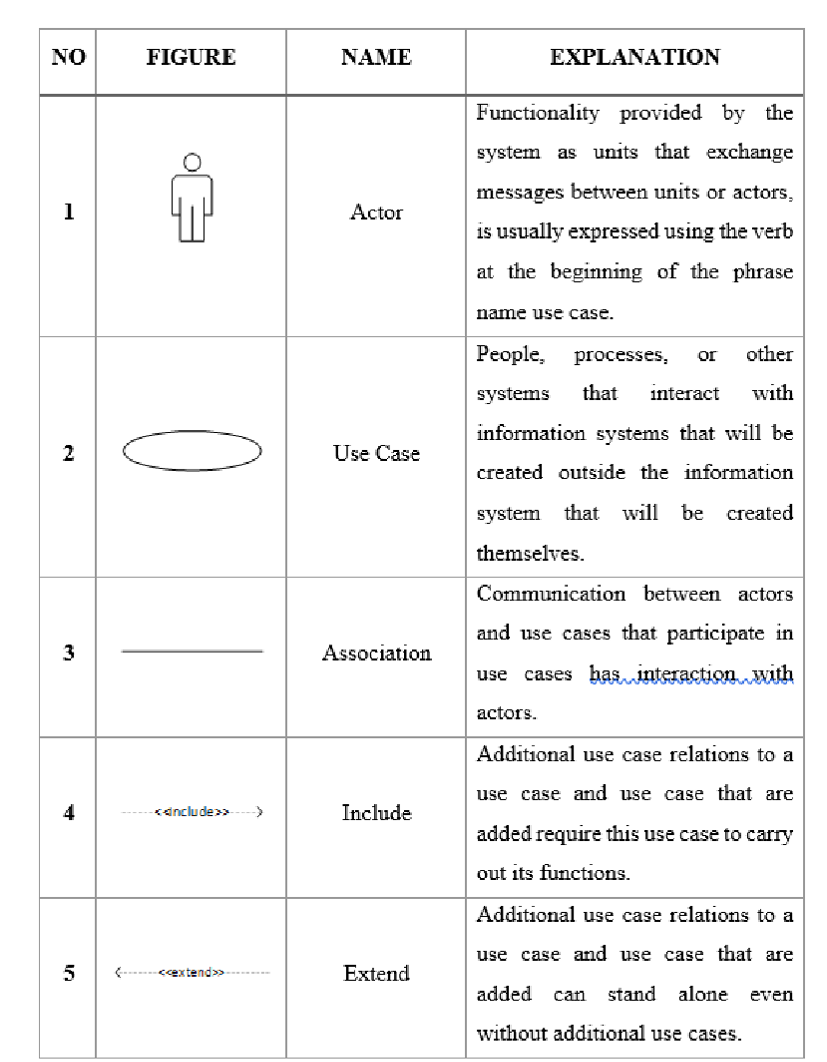
\includegraphics[width=0.85\linewidth]{images/bab-2/uc.png}
  \caption{Simbol ``use case'' diagram}\label{fig:use-case-symbols}\citep{ali2019}
\end{figure}

Selain untuk desain, UML juga digunakan untuk pengujian. Telah dilaporkan bahwa baik diagram UML tunggal maupun ganda digunakan dalam menghasilkan kasus uji, menunjukkan fleksibilitas UML dalam berbagai tahapan pengembangan perangkat lunak. Selain itu, UML telah diperluas dan disesuaikan dalam berbagai cara, seperti dalam pengembangan alat untuk klasifikasi otomatis gambar web dan meningkatkan spesifikasi kebutuhan dalam desain sistem \citep{weriza2022development}.

\subsection{Activity Diagram}
Dalam pengembangan perangkat lunak, diagram aktivitas adalah jenis diagram yang digunakan dalam Unified Modeling Language (UML) untuk menggambarkan aliran aktivitas atau tindakan dalam suatu sistem. Diagram UML berfungsi sebagai satu set notasi universal yang memfasilitasi deskripsi konsep dan kolaborasi di antara pengembang perangkat lunak, arsitek, dan desainer \citep{Shcherban2021}.

\begin{figure}[htbp]
  \centering
  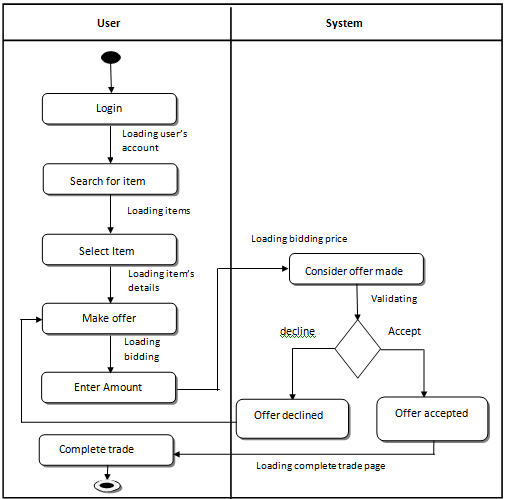
\includegraphics[width=0.85\linewidth]{images/bab-2/act.png}
  \caption{Contoh \emph{Activity Diagram}}\label{fig:activity-diagram-example}\citep{jibrilActivityDiagram}
\end{figure}

Diagram aktivitas UML dilengkapi dengan berbagai simbol yang digunakan untuk merepresentasikan aktivitas, keputusan, ``merge'', dan aliran dalam suatu sistem. Simbol-simbol ini termasuk:
\begin{itemize}
  \item Oval untuk aktivitas.
  \item Berlian untuk keputusan.
  \item Garis panah untuk aliran kendali.
  \item Simbol lain seperti ``swimlanes'' untuk membagi tanggung jawab antara berbagai aktor atau bagian dari sistem.
\end{itemize}
Penggunaan simbol-simbol ini memungkinkan diagram untuk memberikan representasi visual yang jelas dan terstruktur dari proses yang kompleks, sehingga memudahkan pemahaman dan komunikasi antar anggota tim pengembangan. Dengan memahami dan menggunakan simbol-simbol ini dengan benar, desainer dapat memastikan bahwa diagram aktivitas mereka secara akurat mencerminkan logika dan alur kerja dari sistem yang sedang dikembangkan \citep{Casati2002}.

\begin{figure}[htbp]
  \centering
  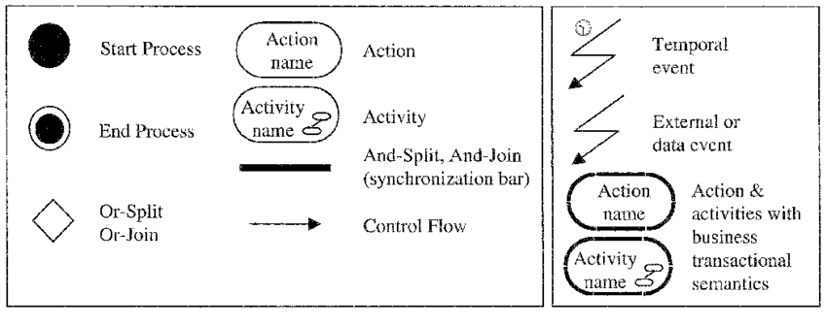
\includegraphics[width=0.85\linewidth]{images/bab-2/act-symbols.png}
  \caption{Simbol-simbol diagram aktivitas}\label{fig:activity-diagram-symbols}\citep{Casati2002}
\end{figure}

Diagram UML, termasuk diagram aktivitas, memainkan peran penting dalam pengembangan perangkat lunak dengan menggambarkan struktur statis dan perilaku dinamis dari sistem perangkat lunak. Diagram ini penting untuk pemodelan orkestrasi layanan, mengekspresikan skenario desain perangkat lunak, dan membantu dalam fase awal siklus hidup pengembangan perangkat lunak \citep{modi2021tool,flores2022empirical}. Selain itu, diagram UML adalah alat standar yang telah diterima secara luas di industri untuk mengembangkan sistem perangkat lunak berbasis objek \citep{weriza2022development}.

\subsection{Sequence Diagram}
Diagram urutan adalah komponen penting dari Unified Modeling Language (UML) yang menyediakan representasi visual tentang bagaimana objek-objek berinteraksi dalam skenario tertentu seiring waktu. Diagram ini diklasifikasikan sebagai diagram interaksi dan sangat efektif dalam menggambarkan perilaku dinamis dari suatu sistem dengan merinci urutan pesan yang dipertukarkan antara objek-objek \citep{huzar2005uml}.

\begin{figure}[htbp]
  \centering
  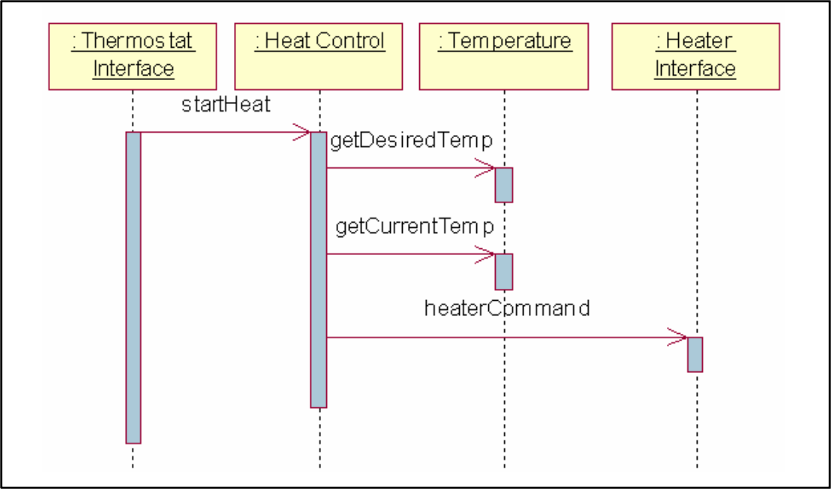
\includegraphics[width=0.85\linewidth]{images/bab-2/sequence.png}
  \caption{Contoh diagram urutan}\label{fig:sequence-diagram-example}\citep{huzar2005uml}
\end{figure}
\singlespacing{}
Dalam diagram urutan, sumbu vertikal mewakili garis waktu, sedangkan sumbu horizontal mencantumkan objek-objek yang terlibat dalam interaksi. Setiap objek digambarkan sebagai ``lifeline'', yaitu garis putus-putus vertikal yang memanjang ke bawah untuk menunjukkan keberadaan objek seiring waktu. Pesan yang dipertukarkan antara objek-objek diwakili oleh panah horizontal, yang diberi anotasi dengan nama pesan dan parameter yang relevan. Urutan pesan ditunjukkan oleh penempatannya sepanjang sumbu vertikal, memungkinkan pemahaman yang jelas tentang aliran kontrol dan data \citep{huzar2005uml}.
\singlespacing{}
Diagram urutan memiliki beberapa tujuan penting dalam pemodelan sistem. Mereka membantu memperjelas interaksi yang diperlukan untuk memenuhi suatu ``use case'' tertentu, sehingga sangat berharga bagi pengembang dan pemangku kepentingan. Dengan memvisualisasikan urutan operasi, diagram ini memfasilitasi komunikasi antar anggota tim dan memberikan pemahaman yang jelas tentang bagaimana berbagai komponen sistem berkolaborasi untuk mencapai fungsionalitas yang diinginkan \citep{huzar2005uml}.
\singlespacing{}
Selain itu, diagram urutan dapat digunakan untuk mengidentifikasi potensi masalah dalam aliran interaksi, seperti pesan yang hilang atau urutan yang salah, sehingga membantu dalam penyempurnaan desain sistem. Diagram ini melengkapi diagram UML lainnya, seperti diagram ``use case'', dengan memberikan pandangan yang lebih rinci tentang interaksi yang terjadi dalam konteks suatu ``use case'' \citep{huzar2005uml}.